\documentclass[conference]{IEEEtran}
\IEEEoverridecommandlockouts

\usepackage{cite}
\usepackage{amsmath,amssymb,amsfonts}
\usepackage{algorithmic}
\usepackage{graphicx}
\usepackage{textcomp}
\usepackage{xcolor}
\usepackage{booktabs}
\usepackage{geometry}

\geometry{
    letterpaper,
    left=0.75in,
    right=0.75in,
    top=0.75in,
    bottom=0.75in
}

% --- Adjust float parameters for tighter text integration ---
\renewcommand{\topfraction}{0.95}
\renewcommand{\textfraction}{0.05}
\renewcommand{\floatpagefraction}{0.85}

\begin{document}

\title{Numerical Investigation of Active Boundary-Layer Momentum Injection on a NACA 0015 Airfoil for Stall Delay}

\author{\IEEEauthorblockN{Authored independently by Muhammad Yousuf Baig}
\IEEEauthorblockA{Email: ybaig1999@gmail.com}
}

\maketitle

\begin{abstract}
This paper presents a 2D Computational Fluid Dynamics (CFD) validation study analyzing the aerodynamic effects of Active Flow Control (AFC) on a symmetrical NACA 0015 airfoil. Utilizing a steady-state pressure-based solver with the Realizable $k-\epsilon$ turbulence model and Enhanced Wall Treatment ($y^+ \approx 1$), the baseline aerodynamic profile was validated against experimental and numerical benchmarks. A parametric Angle of Attack (AoA) sweep from $0^\circ$ to $18^\circ$ was executed at $Re = 1.0 \times 10^6$. Viscous trigonometric coordinate transformations were integrated into the force monitors to eliminate global axis alignment artifacts. In the linear regime ($\alpha < 11^\circ$), the baseline lift curve slope was calculated as $\partial C_L / \partial \alpha = 0.0890/\text{deg}$, closely tracking the benchmark slope of $0.101/\text{deg}$. While the reference literature achieved a $67.1\%$ lift enhancement at $16^\circ$ using high-frequency pulsing Synthetic Jet Actuators (SJA), continuous $40\text{ m/s}$ tangential blowing resulted in an early stall at $14^\circ$ and a $20.88\%$ lift degradation at $16^\circ$ ($C_L$ dropped from $1.1006$ to $0.8708$). This behavior is characterized as the ``Virtual Spoiler'' effect, demonstrating that steady-state blowing acts as a fluidic barrier that trips the boundary layer, thereby confirming the physical necessity of zero-net-mass-flux (ZNMF) high-frequency actuation.
\end{abstract}

\begin{IEEEkeywords}
Computational Fluid Dynamics (CFD), Active Flow Control (AFC), NACA 0015, Stall Delay, Virtual Spoiler Effect, Coordinate Rotation.
\end{IEEEkeywords}

\section{Introduction}
Flow separation over lifting surfaces at high Angles of Attack (AoA) leads to aerodynamic stall, characterized by a sudden loss of lift and a severe increase in pressure drag. Active Flow Control (AFC) via fluidic micro-actuators represents a key mechatronics-fluidic interface for dynamic boundary layer control. 

The primary objective of this study is to validate the baseline open-loop aerodynamic characteristics of a NACA 0015 airfoil and evaluate continuous tangential momentum injection at the leading edge ($x/c = 0.10$), benchmarking the results against established reference literature \cite{mdpi2020}.

\section{Numerical Methodology \& Grid Verification}

\subsection{Domain Geometry \& Operating Conditions}
The domain consists of a 2D symmetrical NACA 0015 airfoil with chord length $c = 0.3\text{ m}$. A $1\text{ mm}$ wide micro-slot ($x/c = 0.10$) is integrated tangentially along the upper surface. The domain employs a structured O-grid topology extending $43.5c$ radially and $30c$ downstream to avoid unphysical far-field reflections. Operating conditions are set to $Re = 1,000,000$ with freestream velocity $U_\infty = 50\text{ m/s}$.

\subsection{Discretization \& Wall Treatment}
Grid independence was verified across a domain of $\sim 107,000$ elements. A total of $584\text{ nodes}$ were assigned along the airfoil surface. Heavy quadrilateral inflation layers were applied to the airfoil and slot walls, maintaining a first cell height between $2.11 \times 10^{-4}c$ and $1.83 \times 10^{-5}c$ to enforce $y^+ \approx 1$. The Realizable $k-\epsilon$ model with Enhanced Wall Treatment (EWT) was selected for boundary layer resolution.

% --- FIGURE 1: Stacked Single-Column (Frees up Page 2) ---
\begin{figure}[htbp]
\centering
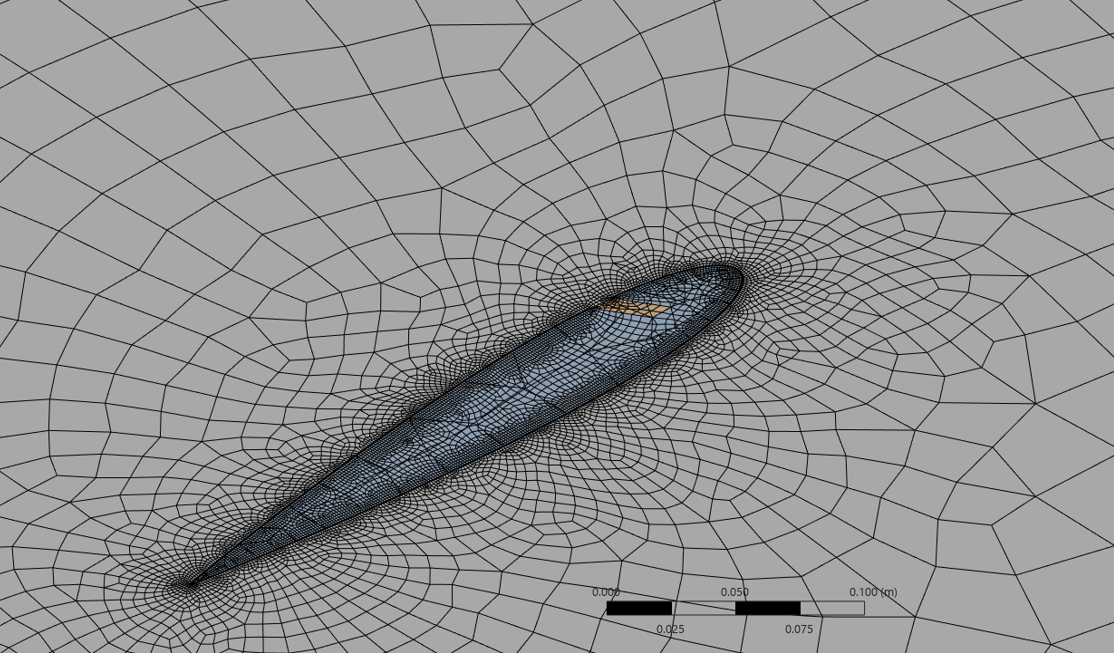
\includegraphics[width=\columnwidth]{mesh.png}
\vspace{0.15cm}
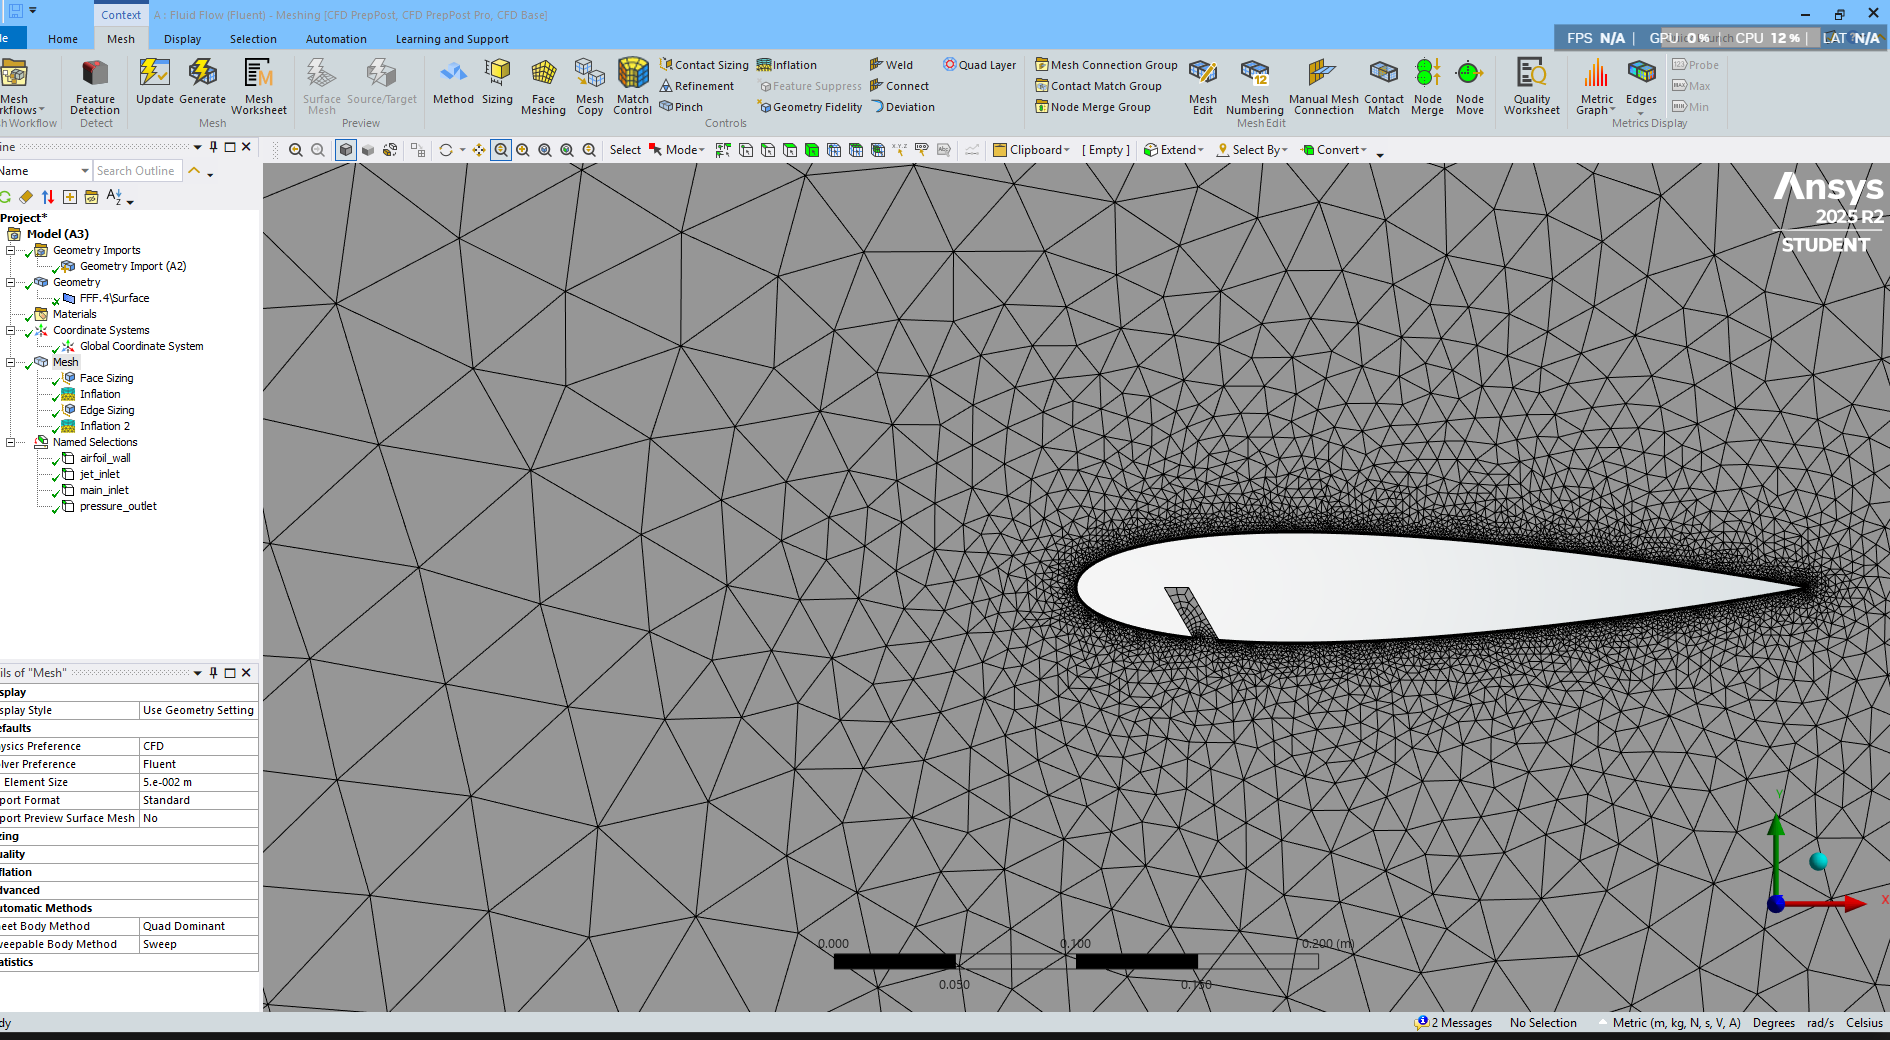
\includegraphics[width=\columnwidth]{mesh-airfoil.png}
\caption{Computational grid discretization: Structured domain O-grid topology (top) and close-up of inflation layers surrounding the NACA 0015 leading edge and micro-slot for $y^+ \approx 1$ boundary layer resolution (bottom).}
\label{fig:mesh_verification}
\end{figure}

% --- FIGURE 2: 4-Panel Contours (Renders top of Page 2) ---
\begin{figure*}[t]
\centering
\begin{minipage}{0.48\textwidth}
  \centering
  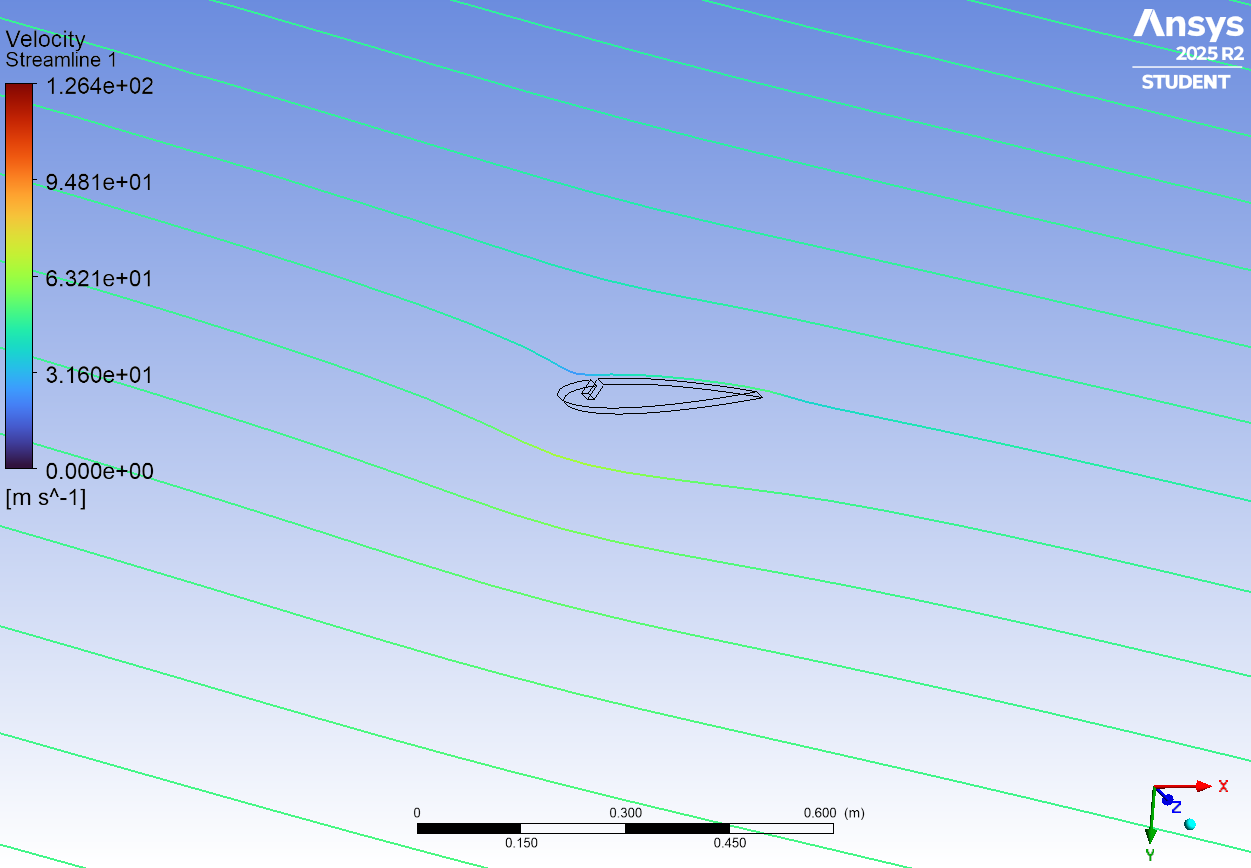
\includegraphics[width=\linewidth]{Stall_OFF_Streamlines_airfoil.png}\\
  \vspace{2pt}\small{(a) Baseline Streamlines ($16^\circ$ Stall)}
\end{minipage}
\hfill
\begin{minipage}{0.48\textwidth}
  \centering
  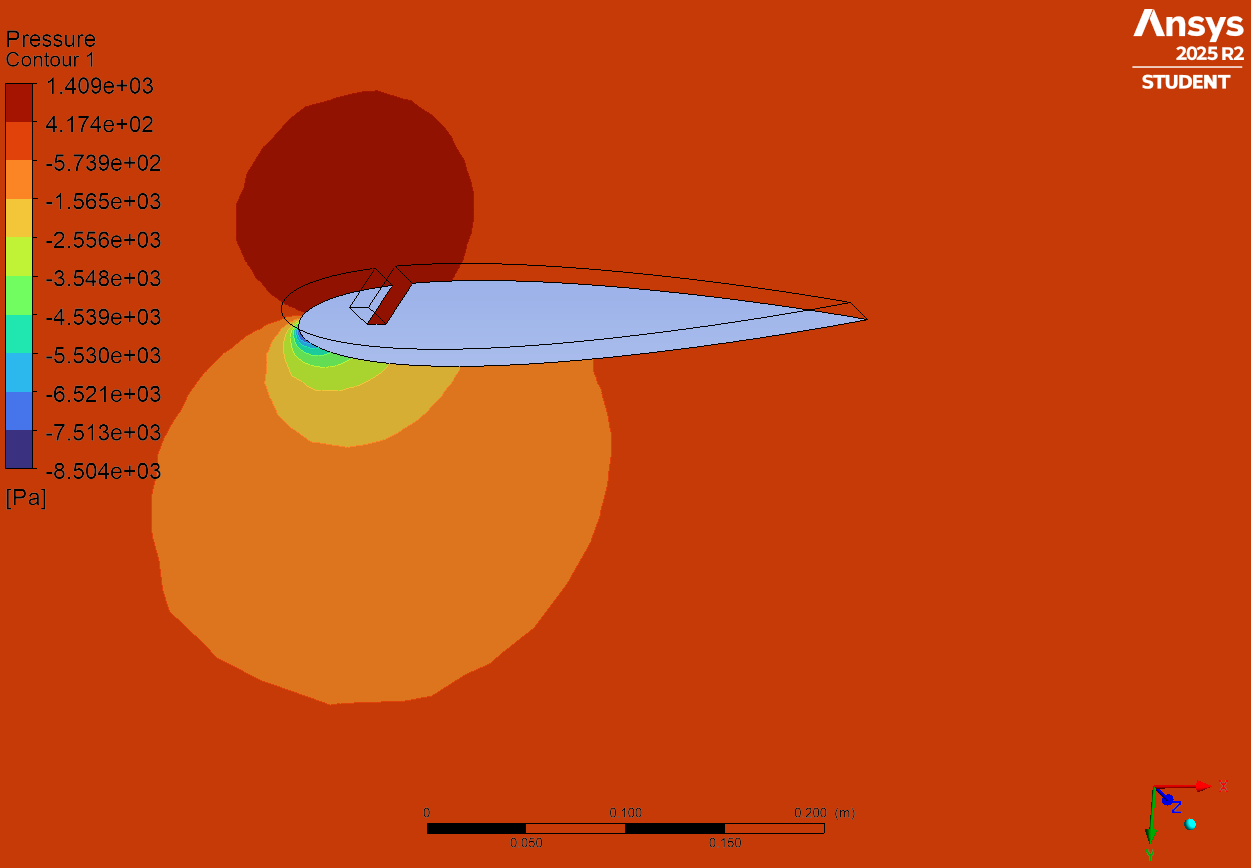
\includegraphics[width=\linewidth]{Stall_OFF_pressure_airfoil.png}\\
  \vspace{2pt}\small{(b) Baseline Pressure Contours ($16^\circ$ Stall)}
\end{minipage}

\vspace{6pt}

\begin{minipage}{0.48\textwidth}
  \centering
  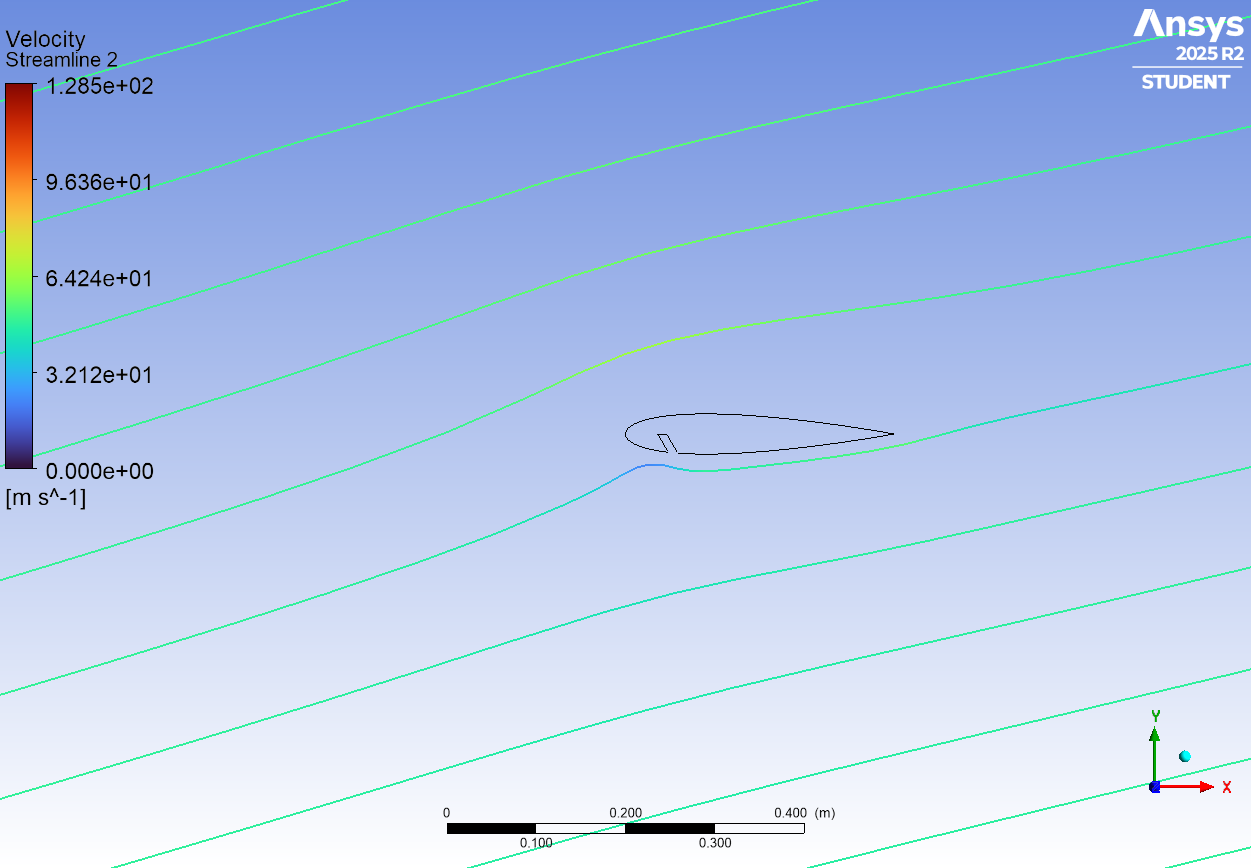
\includegraphics[width=\linewidth]{Stall_ON_Streamlines_airfoil.png}\\
  \vspace{2pt}\small{(c) Actuated Streamlines ($40\text{ m/s}$ Jet)}
\end{minipage}
\hfill
\begin{minipage}{0.48\textwidth}
  \centering
  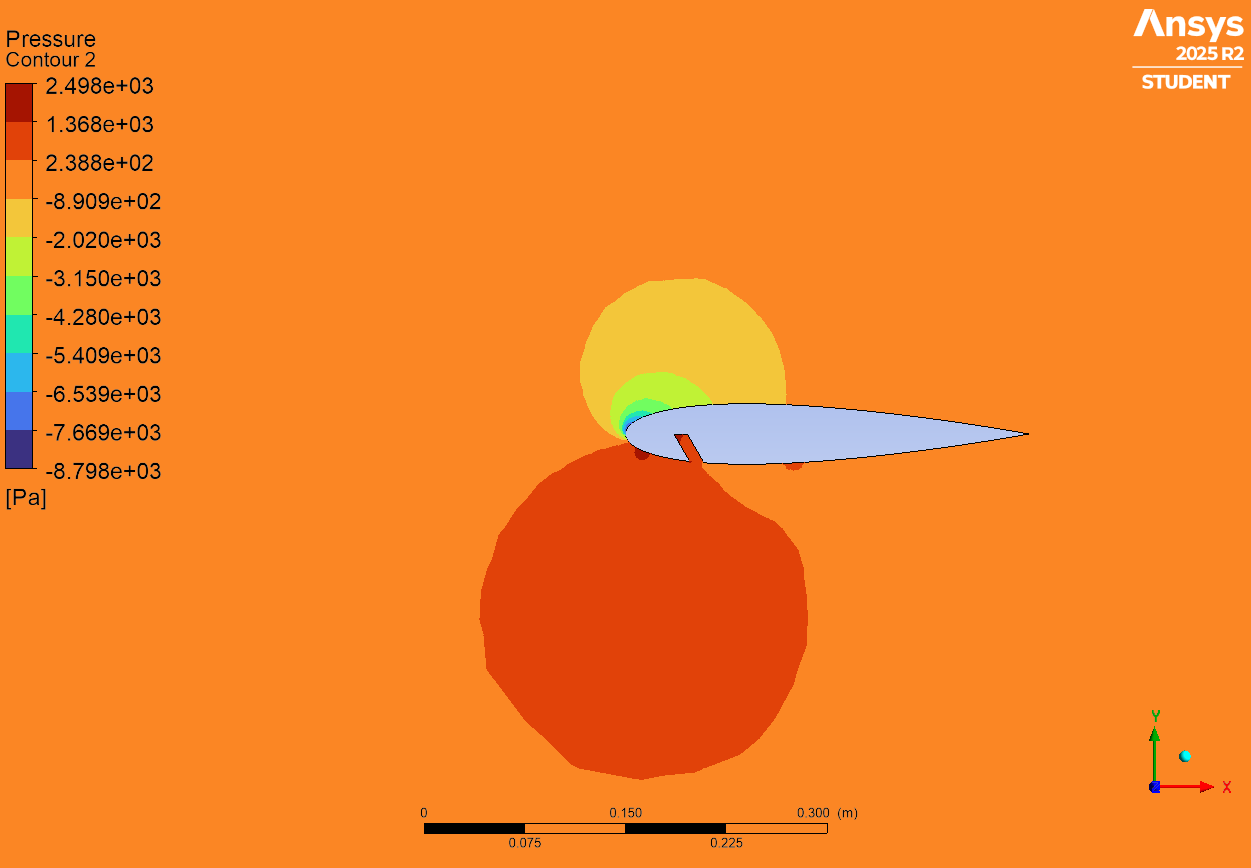
\includegraphics[width=\linewidth]{Stall_on_Pressure_airfoil.png}\\
  \vspace{2pt}\small{(d) Actuated Pressure Contours ($40\text{ m/s}$ Jet)}
\end{minipage}
\caption{Comparative aerodynamic flow field visual validation at $16^\circ$ Angle of Attack: Unactuated baseline trailing-edge separation bubble (top row) vs. continuous momentum injection flow tripping (bottom row).}
\label{fig:contour_comparison}
\end{figure*}

\section{Coordinate Rotation Mathematics}
To automate AoA sweeps ($0^\circ$ to $18^\circ$), oncoming velocity vectors were parameterized as $V_x = U_\infty \cos(\alpha)$ and $V_y = U_\infty \sin(\alpha)$. Because raw Fluent force monitors measure global $X$ and $Y$ Cartesian components, forward projection of the lift vector created unphysical negative drag at lower angles. True body-fixed lift ($C_L$) and drag ($C_D$) were resolved via trigonometric transformations:

\begin{equation}
\text{True } C_{L,\text{OFF}} = P_3 \cos\left(P_4 \frac{\pi}{180}\right) - P_2 \sin\left(P_4 \frac{\pi}{180}\right)
\end{equation}
\begin{equation}
\text{True } C_{D,\text{OFF}} = P_2 \cos\left(P_4 \frac{\pi}{180}\right) + P_3 \sin\left(P_4 \frac{\pi}{180}\right)
\end{equation}
\begin{equation}
\text{True } C_{L,\text{ON}} = P_7 \cos\left(P_5 \frac{\pi}{180}\right) - P_6 \sin\left(P_5 \frac{\pi}{180}\right)
\end{equation}
\begin{equation}
\text{True } C_{D,\text{ON}} = P_6 \cos\left(P_5 \frac{\pi}{180}\right) + P_7 \sin\left(P_5 \frac{\pi}{180}\right)
\end{equation}

\noindent where $\alpha = P_4, P_5$, raw drag $C_{D,\text{raw}} = P_2, P_6$, and raw lift $C_{L,\text{raw}} = P_3, P_7$.

\section{Results \& Physical Discussion}

\begin{table}[htbp]
\caption{Comparative Aerodynamic Metrics Summary}
\begin{center}
\begin{tabular}{lccc}
\toprule
\textbf{Metric / Parameter} & \textbf{Baseline} & \textbf{Actuated} & \textbf{Target Benchmark} \\
\midrule
Linear Slope $\partial C_L/\partial \alpha$ & $0.0890/\text{deg}$ & -- & $0.101/\text{deg}$ \\
Stall Angle ($\alpha_{\text{stall}}$) & $16^\circ$ & $14^\circ$ & $> 16^\circ$ \\
Peak $C_L$ at $16^\circ$ & $1.1006$ & $0.8708$ & $1.3150$ \\
$C_L$ Change at $16^\circ$ & -- & $-20.88\%$ & $+67.1\%$ \\
\bottomrule
\end{tabular}
\end{center}
\end{table}

\subsection{Baseline Aerodynamic Validation}
In the attached linear regime ($\alpha < 11^\circ$), the calculated lift curve slope of $0.0890/\text{deg}$ validates the numerical mesh against thin-airfoil theory ($0.101/\text{deg}$). The baseline unforced wing exhibits classic trailing-edge stall behavior at $\alpha = 16^\circ$. As the adverse pressure gradient intensifies along the suction surface, the boundary layer detaches near the trailing edge, forming a large turbulent recirculation bubble that limits maximum lift to $C_{L,\text{max}} = 1.1006$.

% --- FIGURE 3: Enlarged Actuator Graphs (Renders top of Page 3) ---
\begin{figure*}[t]
\centering
\begin{minipage}{0.495\textwidth}
  \centering
  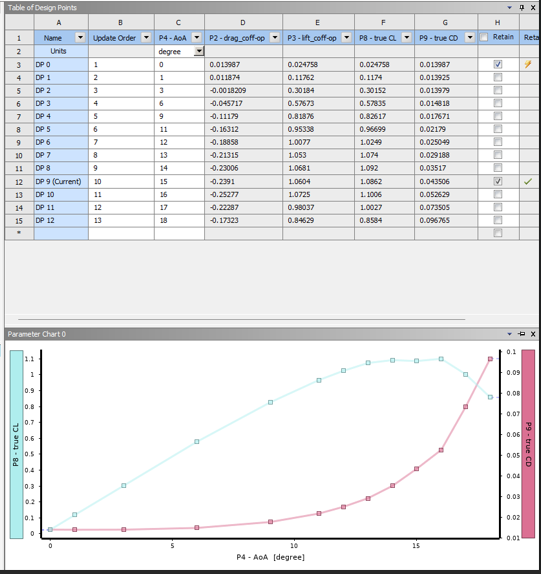
\includegraphics[width=\linewidth]{actuator_off_grapgh1.png}
  \vspace{2pt}\small{(a) Baseline Actuator OFF response and design table.}
\end{minipage}
\hfill
\begin{minipage}{0.495\textwidth}
  \centering
  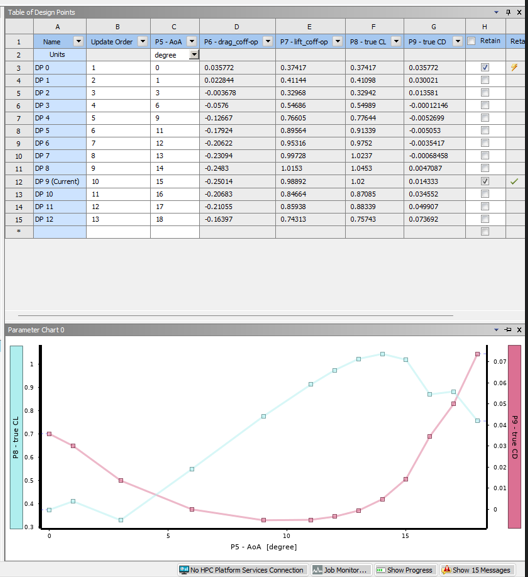
\includegraphics[width=\linewidth]{actuator_on_grraph1.png}
  \vspace{2pt}\small{(b) Actuator ON continuous blowing response.}
\end{minipage}
\caption{Side-by-side aerodynamic performance validation curves ($0^\circ$ to $18^\circ$ AoA): Baseline Actuator OFF performance curves and data table (left) vs. Actuator ON continuous $40\text{ m/s}$ blowing response (right).}
\label{fig:lift_drag_comparison}
\end{figure*}

\subsection{Fluid Dynamics of the Virtual Spoiler Effect}
Under continuous tangential blowing at $V_j = 40\text{ m/s}$ ($C_\mu = 0.0064$), two distinct fluid phenomena were observed:
\begin{enumerate}
    \item \textbf{Zero-Degree Coanda Circulation Enhancement:} At $\alpha = 0^\circ$, high-velocity air injected along the upper surface accelerates local fluid, reducing static pressure via the Coanda effect. This generates an asymmetric pressure differential, yielding an initial lift coefficient of $C_L = 0.374$ at zero incidence.
    \item \textbf{High-Angle Flow Tripping (Virtual Spoiler):} At high angles of attack ($\alpha \ge 14^\circ$), the continuous momentum jet encounters a severe adverse pressure gradient. Instead of energizing the boundary layer, the steady jet stream creates a thick localized stagnation zone that acts as a physical barrier---a ``Virtual Spoiler.'' This fluidic wall increases displacement thickness, trips the shear layer prematurely, and shifts flow separation forward to $x/c \approx 0.15$. Consequently, peak lift drops by $20.88\%$ at $\alpha = 16^\circ$ ($C_L$ falling from $1.1006$ to $0.8708$) alongside a significant increase in pressure drag.
\end{enumerate}

\subsection{Physical Implications for Active Flow Control Design}
The numerical results highlight a fundamental limitation of steady-state momentum injection in open-loop active flow control configurations. While continuous blowing provides low-AoA circulation gains through surface jet vectoring, it severely degrades aerodynamic authority near the stall threshold. 

To achieve effective boundary layer delay without inducing virtual spoiler penalties, fluidic actuation must utilize zero-net-mass-flux (ZNMF) high-frequency pulsing, such as Synthetic Jet Actuators (SJAs). Pulsed momentum injection introduces discrete coherent vortex structures that promote turbulent mixing between the outer freestream flow and the inner boundary layer without forming a continuous fluidic blockage.

\section{Conclusion}
This 2D CFD validation study successfully established the baseline aerodynamics of a NACA 0015 airfoil, capturing a linear lift slope of $0.0890/\text{deg}$ and baseline stall at $\alpha = 16^\circ$. Continuous $40\text{ m/s}$ tangential momentum injection resulted in a virtual spoiler effect at high angles of attack, causing premature separation at $14^\circ$ and a $20.88\%$ reduction in peak lift. These findings confirm the physical necessity of unsteady, high-frequency pulsed actuation for effective active aerodynamic separation control.

\begin{thebibliography}{00}
\bibitem{mdpi2020} MDPI Fluids, ``NARMAX Identification Based Closed-Loop Control of Flow Separation over NACA 0015 Airfoil,'' \textit{Fluids}, vol. 5, no. 1, p. 100, 2020.
\end{thebibliography}

\end{document}